\documentclass{article}

\usepackage{microtype}
\usepackage{graphicx}
\usepackage{booktabs}
\usepackage{multirow}
\usepackage{hyperref}
\newcommand{\theHalgorithm}{\arabic{algorithm}}
\usepackage[accepted]{icml2024}

\usepackage{amsmath}
\usepackage{amssymb}
\usepackage{mathtools}
\usepackage[capitalize,noabbrev]{cleveref}
\usepackage[section]{placeins}

\graphicspath{{../}{../figures/}}

\setlength{\intextsep}{5pt plus 1pt minus 1pt}
\setlength{\textfloatsep}{6pt plus 1pt minus 1pt}
\setlength{\floatsep}{6pt plus 1pt minus 1pt}
\setlength{\dbltextfloatsep}{6pt plus 1pt minus 1pt}
\setlength{\dblfloatsep}{6pt plus 1pt minus 1pt}
\setlength{\abovecaptionskip}{3pt}
\setlength{\belowcaptionskip}{2pt}

\emergencystretch=2em
\tolerance=2000
\hyphenpenalty=50
\sloppy

\renewcommand{\arraystretch}{1.10}
\newcommand{\best}[1]{\textbf{#1}}

\icmltitlerunning{Human-in-the-Loop LLM Workflow for Research Roadmap Curation}

\begin{document}

\twocolumn[
\icmltitle{A Human-in-the-Loop LLM Workflow for Research Roadmap Curation}

\begin{icmlauthorlist}
\icmlauthor{Prathamesh Joshi}{vizuara}
\icmlauthor{Abraar}{vizuara}
\icmlauthor{Naman Dwivedi}{vizuara}
\icmlauthor{Dr Raj Dandekar}{vizuara}
\icmlauthor{Dr Rajat Dandekar}{vizuara}
\icmlauthor{Dr Sreedath Dandekar}{vizuara}
\end{icmlauthorlist}

\icmlaffiliation{vizuara}{Vizuara AI Labs}

\icmlcorrespondingauthor{Prathamesh Joshi}{prathamesh@vizuara.com}
\icmlkeywords{Large Language Models, Human-in-the-Loop, Research Planning, Workflow}

\vskip 0.3in
]

\printAffiliationsAndNotice{}

\begin{abstract}
Early-stage research often begins with vague ideas that are not yet
executable. Converting a broad interest into a concrete project requires
research questions, literature directions, datasets, baselines, evaluation
metrics, ablations, milestones, risks, and a realistic contribution claim.
Large language models (LLMs) can assist with this planning stage, but unstructured
prompting tends to produce roadmaps that are fluent yet generic, hard to
verify, or poorly scoped. We present a human-in-the-loop LLM workflow for
research roadmap curation. Given a raw research idea, the workflow generates
a structured roadmap artifact that is reviewed, revised, and approved by a
human reviewer, who may be the researcher themselves, a mentor, an
instructor, a collaborator, or a domain expert. The workflow is
model-agnostic; our prototype conditions an LLM backend on reference
templates, optionally retrieves relevant literature, emits LaTeX, compiles
a PDF, and exposes the result for review through an asynchronous job queue.
We evaluate the workflow with a blind human preference study in which $40$
evaluators rated four anonymized roadmap variants for the same idea on
completeness, feasibility, specificity, experiment design, and research
potential. \textbf{Of the $40$ evaluators, $34$ ($85\%$) selected the
roadmap produced by our workflow as the one they would adopt overall},
versus $6$ combined for the three unstructured ChatGPT baselines. The
result is consistent with the hypothesis that schema-constrained generation
under human review yields more usable first-pass research plans than
one-shot prompting, while keeping a human accountable for feasibility and
novelty.
\end{abstract}

\section{Introduction}
\label{sec:intro}

Early-stage research projects often fail before any experiment is run.
The initial idea is too broad, the dataset is unclear, the baselines are
missing, the evaluation metrics do not match the question, or the
expected contribution is overclaimed. This pattern is especially common
in research bootcamps, undergraduate research programs, industry
training cohorts, and early-stage graduate projects, where participants
begin with enthusiasm but limited experience converting a broad interest
into an executable plan.

A vague idea is not yet a research project. Statements such as ``I want
to work on multimodal RAG'', ``I want to apply reinforcement learning to
retrieval'', or ``I want to use scientific machine learning for physical
systems'' are useful starting points, but they do not specify what
should be built, what should be compared, what evidence should be
collected, or what claim the final paper or report could defend. To
become actionable, such ideas must be transformed into structured
roadmaps that include research questions, literature directions,
datasets, baselines, metrics, ablations, weekly milestones, risks,
deliverables, and a minimum viable claim. This transformation is
typically performed by a human mentor, instructor, supervisor, or domain
expert, and it does not scale: in a cohort with many students, mentors
must repeatedly convert loosely stated interests into detailed project
plans, and the bottleneck is not the document itself but the judgment
required to keep it specific, feasible, experimentally sound, and
appropriately scoped.

Large language models (LLMs) are a natural fit for this stage. However,
one-shot prompting is often insufficient. A generic prompt such as
``generate a 12-week research roadmap for this idea'' produces fluent
output that may omit baselines, suggest unrealistic datasets, fail to
define measurable success criteria, or overstate the novelty of the
project. The surface fluency of LLM-generated prose can also make weak
plans appear more credible than they are. Our central question is
therefore: \emph{can a structured, human-reviewed LLM workflow help
convert vague research ideas into executable roadmaps more reliably
than unstructured prompting?}

We present a human-in-the-loop LLM workflow for research roadmap
curation. Given a raw research idea, the workflow generates a structured
roadmap artifact, which is then routed to a human reviewer who can
inspect, revise, or approve it. The reviewer may be the original
researcher, a mentor, an instructor, a supervisor, a collaborator, or a
domain expert. The workflow is model-agnostic: it can be instantiated
using API-based models, coding agents, or local models, as long as the
backend supports structured generation and artifact creation. Our
prototype processes requests asynchronously, conditions on reference
templates, optionally retrieves relevant literature, emits LaTeX,
compiles a PDF, and exposes the result for review.

We evaluate the workflow with a blind human preference study. For one
research idea, four anonymized roadmap variants were generated:
variants A, B, and D from three different unmodified ChatGPT versions
prompted in an unstructured way, and variant C from our workflow.
Forty evaluators rated all four roadmaps along five dimensions
(completeness, feasibility, specificity and actionability, experiment
design quality, and research potential) and recorded a single overall
preference. \textbf{$34$ of $40$ evaluators ($85\%$) selected variant C
overall}, with the remaining $6$ ($15\%$) distributed across the three
unstructured baselines.

We make three contributions:
\begin{itemize}
    \item We formulate research-roadmap generation as a
    human-in-the-loop workflow rather than a one-shot generation task,
    and articulate why the human stays in the loop after generation
    rather than only at prompt time.
    \item We introduce a roadmap schema that decomposes early-stage
    research planning into twelve concrete components, including
    research questions, datasets, baselines, metrics, ablations, risks,
    milestones, and a minimum viable claim, so that quality stops
    depending on surface fluency.
    \item We describe and run a blind human-preference evaluation
    protocol that compares four anonymized roadmap variants for a
    shared research idea across five quality dimensions, and report a strong overall
    preference for the schema-constrained, human-reviewed variant.
\end{itemize}

The rest of the paper is organized as follows.
Section~\ref{sec:related} positions the workflow against related work on
LLM-assisted research and structured prompting.
Section~\ref{sec:method} describes the workflow, the roadmap schema, and
the asynchronous job lifecycle.
Section~\ref{sec:eval} defines the evaluation protocol and study setup.
Section~\ref{sec:results} reports the preference results, and
Sections~\ref{sec:discussion} and \ref{sec:limitations} discuss
implications and threats to validity.

\section{Related Work}
\label{sec:related}

\paragraph{LLMs as research assistants and autonomous scientists.}
A growing body of work investigates large language models in roles
ranging from open-ended idea generation and hypothesis proposal to
end-to-end autonomous scientists that orchestrate experiments and
write papers \cite{lu2024aiscientist, baek2024researchagent, yang2023largelanguagemodelshypotheses}. These systems are ambitious
about scope, often aiming to produce or evaluate full research outputs.
Their evaluations focus on the quality of the produced artifact (a
paper, a hypothesis, or an experiment) rather than on the planning
artifact that precedes execution. Our framing is narrower and more
operational: the LLM is a planning assistant that drafts an executable
roadmap, and the human keeps responsibility for feasibility, novelty
calibration, and scientific correctness.

\paragraph{Structured and schema-constrained generation.}
Prompting strategies that impose structure on LLM output (chain-of-thought
\cite{wei2022chainofthought},
self-consistency \cite{wang2023selfconsistency}, and tree-of-thoughts
\cite{yao2024treeofthoughts}) consistently improve reliability on
reasoning-heavy tasks. Schema- or grammar-constrained decoding
\cite{willard2023grammarconstrained, geng2024constraineddecoding}
goes further by forcing outputs into a parseable format. Our roadmap
schema is a coarse-grained instance of the same idea applied to research
planning: rather than constrain syntax, we constrain the set of
components a roadmap must populate (questions, datasets, baselines,
metrics, ablations, milestones, risks, deliverables, minimum viable
claim) so that quality stops depending on surface fluency.

\paragraph{Human-in-the-loop and mixed-initiative AI.}
Mixed-initiative systems with explicit human-AI interaction have a long
history in HCI \cite{horvitz1999mixedinitiative, amershi2019humanaiinteraction}. Recent work specifically on
human-in-the-loop LLM workflows studies prompt iteration
\cite{zamfirescupereira2023nonexperts},
co-writing and editing assistants \cite{lee2022coauthor, yuan2022wordcraft}, and AI-assisted code review and refactoring
\cite{mozannar2024readingbetween}. The shared lesson is that the human
contribution is not just the initial prompt but the editorial judgment
applied after generation. Our workflow exposes this point of judgment
explicitly through a reviewable artifact and an approve/revise state
transition, rather than relying on free-form chat turns.

\paragraph{Human preference evaluation of LLM output.}
Pairwise and small-batch human preference judgments are now a standard
evaluation primitive for LLM outputs, both for alignment training
\cite{ouyang2022instructgpt, bai2022rlhf} and for benchmarking deployed
models \cite{chiang2024chatbotarena, zheng2023llmasajudge}. We adopt the
same primitive (blind human selection among anonymized variants) but
apply it to the relatively unstudied artifact of a research roadmap, and
we ask evaluators to rate five quality dimensions chosen specifically
for executability rather than for fluency or helpfulness.

\paragraph{Existing structured-planning artifacts.}
The twelve-component schema is not derived from a vacuum; it is closest
in spirit to mentor checklists used in research bootcamps, to
proposal-style templates such as the NeurIPS Datasets and Benchmarks
checklist and ML reproducibility checklists \cite{pineau2021reproducibility},
and to the proposal scaffolds embedded in modern note-taking and project
management tools (Notion AI templates, Airtable research planners, and
similar). These artifacts predate the workflow described here and
already encode many of the same components (research questions,
datasets, baselines, milestones, deliverables). Our contribution
relative to that body of practice is twofold: we bind the schema to a
generation backend so the components are populated by an LLM rather
than left as empty fields, and we put the populated artifact through an
explicit reviewable revision loop. The schema itself overlaps
substantially with prior planning rubrics; the workflow surrounding it
is what is new.


\paragraph{Distinguishing this work.}
The closest prior art is the union of structured prompting,
human-in-the-loop writing assistants, and existing research-planning
checklists and templates. Structured prompting work shows
that constraining the output space helps; human-in-the-loop writing
work shows that retaining a human review step matters; autonomous
science work shows that LLMs can produce research-shaped artifacts.
None of these threads directly studies the early-stage planning
artifact, namely an executable research roadmap, as a deliverable in
its own right. Our contribution is to specify the schema, build a
review-and-revision workflow around it, and evaluate the resulting
roadmaps with a blind human preference study against unstructured
prompting baselines.

\section{Method}
\label{sec:method}

We define a research roadmap as an execution-oriented planning artifact
that transforms a broad research idea into a concrete project plan. A
good roadmap should help a researcher understand what to read, what to
implement, what to compare, how to evaluate progress, and what claim the
final project may support. Unlike a literature review or a project
proposal, a roadmap is explicitly operational: it should describe both
the intellectual structure of the project and its execution structure,
including what needs to happen in week one, week two, and so on.

The central design choice is to separate generation from approval. The
LLM drafts the roadmap; a human reviewer decides whether the roadmap is
usable, and revises it through a feedback loop until it is. This loop is
what distinguishes the workflow from one-shot prompting.

\subsection{Workflow Overview}
\label{sec:method:workflow}

The workflow has five stages, illustrated in
Figure~\ref{fig:fig-workflow}: idea submission, structured generation,
artifact creation, human review, and revision-or-delivery. A user submits
a raw research idea together with optional constraints (target duration,
researcher background, preferred domain, tool or dataset constraints,
and a target output type such as paper, report, codebase, or
presentation). An LLM backend generates a roadmap conditioned on a fixed
schema (Section~\ref{sec:method:schema}) and reference templates. The
roadmap is converted into a reviewable artifact, in our prototype a
LaTeX-source-plus-PDF document. A human reviewer inspects the artifact
and either approves it or returns it with revision requests. On
revision, the workflow regenerates or edits the roadmap with reviewer
feedback in context; on approval, the roadmap is delivered or used
directly.

\begin{figure}[t]
  \centering
  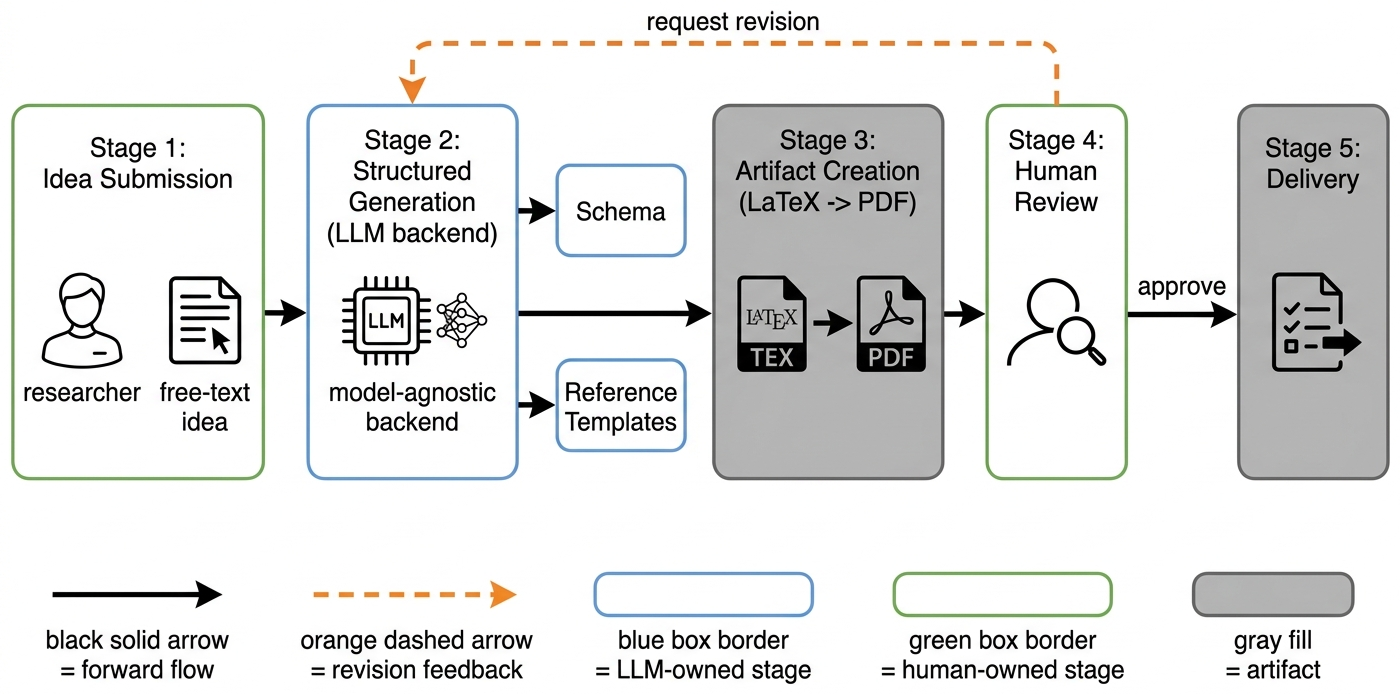
\includegraphics[width=0.95\linewidth]{figures/fig-workflow.png}
  \caption{End-to-end human-in-the-loop roadmap-curation workflow. A raw
  research idea flows through schema-constrained LLM generation, artifact
  creation, and human review. The reviewer can approve the roadmap for
  delivery or route it back through the revision loop (orange dashed
  arrow). The human reviewer remains responsible for feasibility,
  novelty calibration, and scientific correctness.}
  \label{fig:fig-workflow}
\end{figure}

The reviewer is not only the person who writes the initial prompt; the
human remains involved after generation, when quality judgments are
required. This makes the workflow human-in-the-loop rather than merely
human-initiated. The reviewer may be the original researcher, a faculty
advisor, a bootcamp mentor, a teaching assistant, a lab lead, or a domain
expert. The core requirement is not a specific role but a decision point
where a human accepts responsibility for the final plan.

\subsection{Roadmap Schema}
\label{sec:method:schema}

The LLM is not asked to freely brainstorm. Each generated roadmap is
constrained to populate a fixed set of components, grouped into three
families (Figure~\ref{fig:fig-schema}). The \emph{scoping} family
defines what the project is and is not: research scope, research
questions, literature directions, and a minimum viable claim. The
\emph{methodology} family defines what evidence the project will use
and how the technical approach will be evaluated: dataset or environment
plan, methodology, baselines, metrics, and ablations. The
\emph{execution} family converts the project into operational steps:
weekly milestones, risks and mitigations, and concrete deliverables.

\begin{figure}[t]
  \centering
  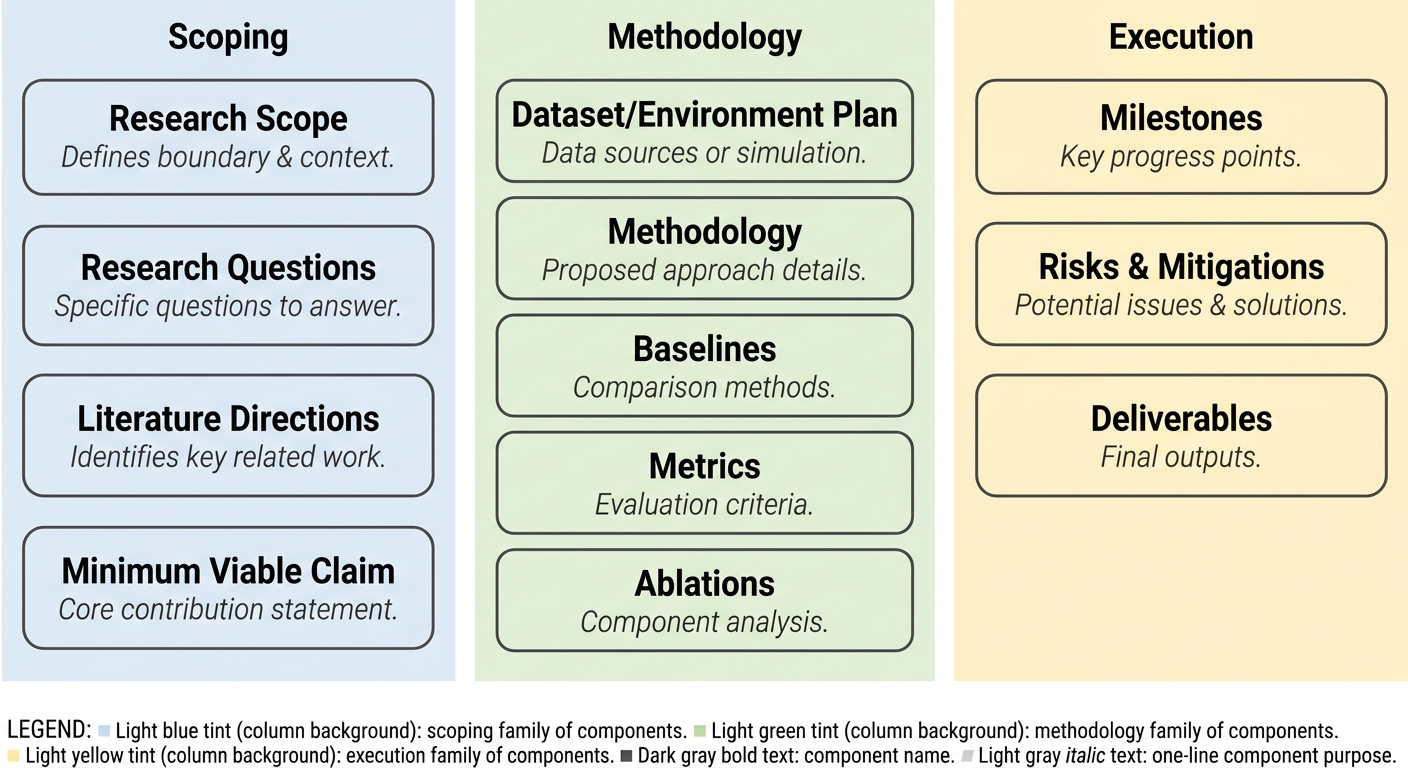
\includegraphics[width=0.95\linewidth]{figures/fig-schema.png}
  \caption{Twelve required components of the roadmap schema, organized
  into a scoping family, a methodology family, and an execution family.
  Schema-constrained generation forces the LLM to populate every
  component rather than producing free-form prose.}
  \label{fig:fig-schema}
\end{figure}

Reference templates are concrete instances of past roadmaps that
follow the schema and ship with the workflow; the LLM backend is
shown one or more matching templates as few-shot exemplars before it
drafts a new roadmap, which steers the surface form toward the schema
without dictating the substantive content. The schema itself is
intentionally coarse-grained. It does not prescribe how
each component is written; it only requires that each component be
present and substantive. The twelve components and three-family grouping are a design choice
distilled from the mentor checklists used in the bootcamp from which
the evaluator cohort is drawn, rather than a derivation from prior
planning literature. The intent is to make roadmap quality less
dependent on surface fluency. A roadmap is not strong merely because it
reads well; it must specify how the project can actually be executed and
evaluated. Concretely, the schema makes weak baselines, missing metrics,
and unstated risks visible to a reviewer at a glance, because the slot
for that component is empty or visibly thin.

\subsection{Model-Agnostic Asynchronous Backend}
\label{sec:method:backend}

The workflow is independent of any single LLM provider. The backend can
be any model or agent that supports structured generation and optional
tool use, including API-based models, coding agents, or local models.
Our prototype uses an asynchronous worker architecture: a roadmap
request is stored as a job, picked up by a worker that calls the LLM
backend with the schema and templates, optionally retrieves relevant
literature, emits LaTeX source, and compiles a PDF that is exposed to
the reviewer.

\begin{figure}[t]
  \centering
  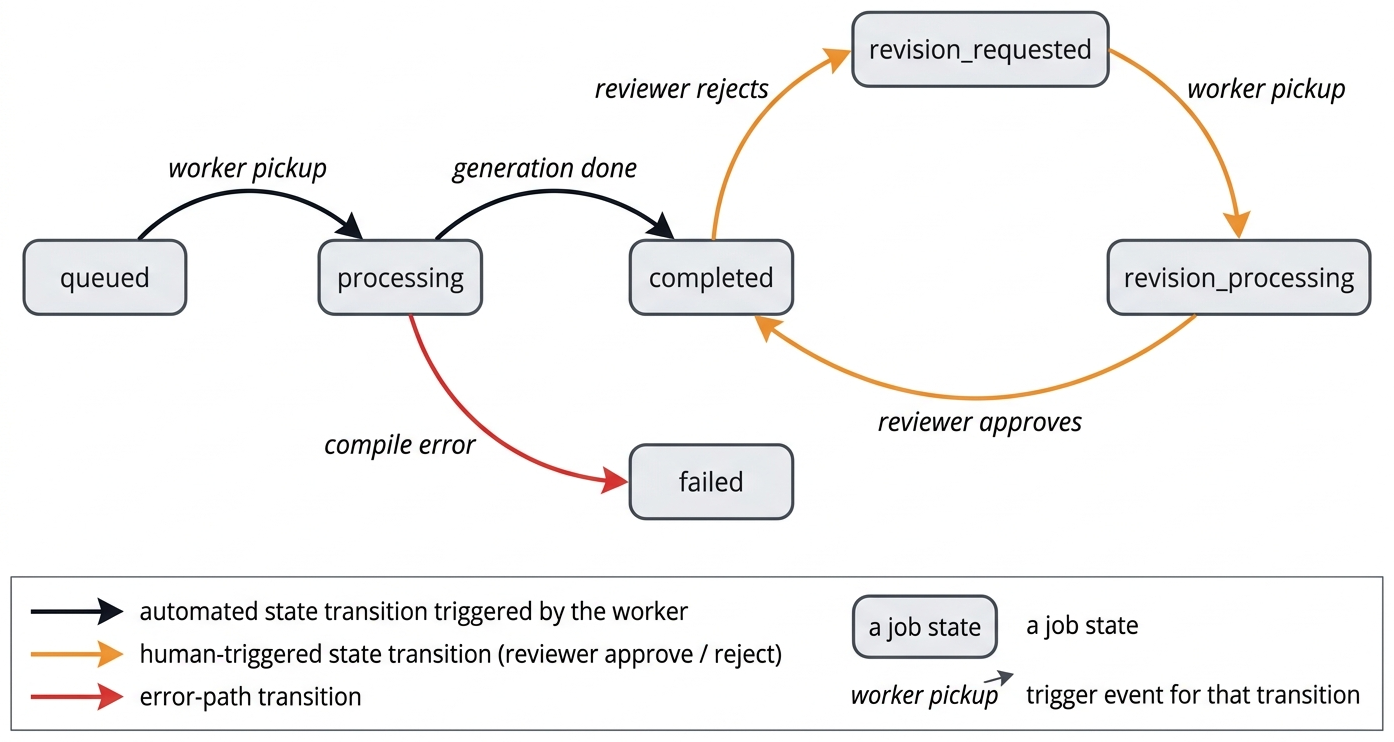
\includegraphics[width=0.95\linewidth]{figures/fig-job-states.png}
  \caption{Job state machine for a roadmap request. The linear path
  \textsf{queued} $\rightarrow$ \textsf{processing} $\rightarrow$
  \textsf{completed} is automated. The cycle
  \textsf{completed} $\rightarrow$ \textsf{revision\_requested}
  $\rightarrow$ \textsf{revision\_processing} $\rightarrow$
  \textsf{completed} is the explicit human-in-the-loop hook that
  distinguishes the workflow from one-shot chat.}
  \label{fig:fig-job-states}
\end{figure}

The job state machine (Figure~\ref{fig:fig-job-states}) supports six
states: \textsf{queued}, \textsf{processing}, \textsf{completed},
\textsf{failed}, \textsf{revision\_requested}, and
\textsf{revision\_processing}. The presence of a dedicated
\textsf{revision\_requested} state, separate from \textsf{processing},
makes the human review point a first-class concept rather than a chat
turn. Long-running generation, compile errors, and asynchronous
revisions all become observable transitions rather than hidden behavior.
The job queue is not a scientific contribution by itself; it is the
implementation mechanism that lets the workflow behave like a real
review-and-revision system instead of a synchronous chat interaction.

\subsection{Human Review Criteria}
\label{sec:method:review}

Human review is necessary because roadmap quality depends on judgments
that LLMs cannot reliably make alone. A roadmap may appear polished
while still being unrealistic, too broad, weakly evaluated, or
scientifically shallow. The reviewer is asked to check whether: the
research question is precise, the proposed dataset is accessible, the
baselines are appropriate, the metrics are measurable, the milestones
are realistic, the risks are honestly stated, and the minimum viable
claim is not overconfident. If any of these checks fails, the reviewer
moves the job into \textsf{revision\_requested} with feedback; the
feedback is provided as context to the next generation or editing
cycle, and the loop repeats until the reviewer approves the roadmap or
abandons it.

\section{Evaluation Protocol}
\label{sec:eval}

We evaluate the workflow with a blind human preference study. The study
compares multiple roadmap variants generated for the \emph{same}
research idea and the \emph{same} input description. Holding the topic
fixed across variants controls for topic preference and isolates
roadmap-quality judgments from idea preference. The study design is
illustrated in Figure~\ref{fig:fig-study-design}.

\begin{figure}[t]
  \centering
  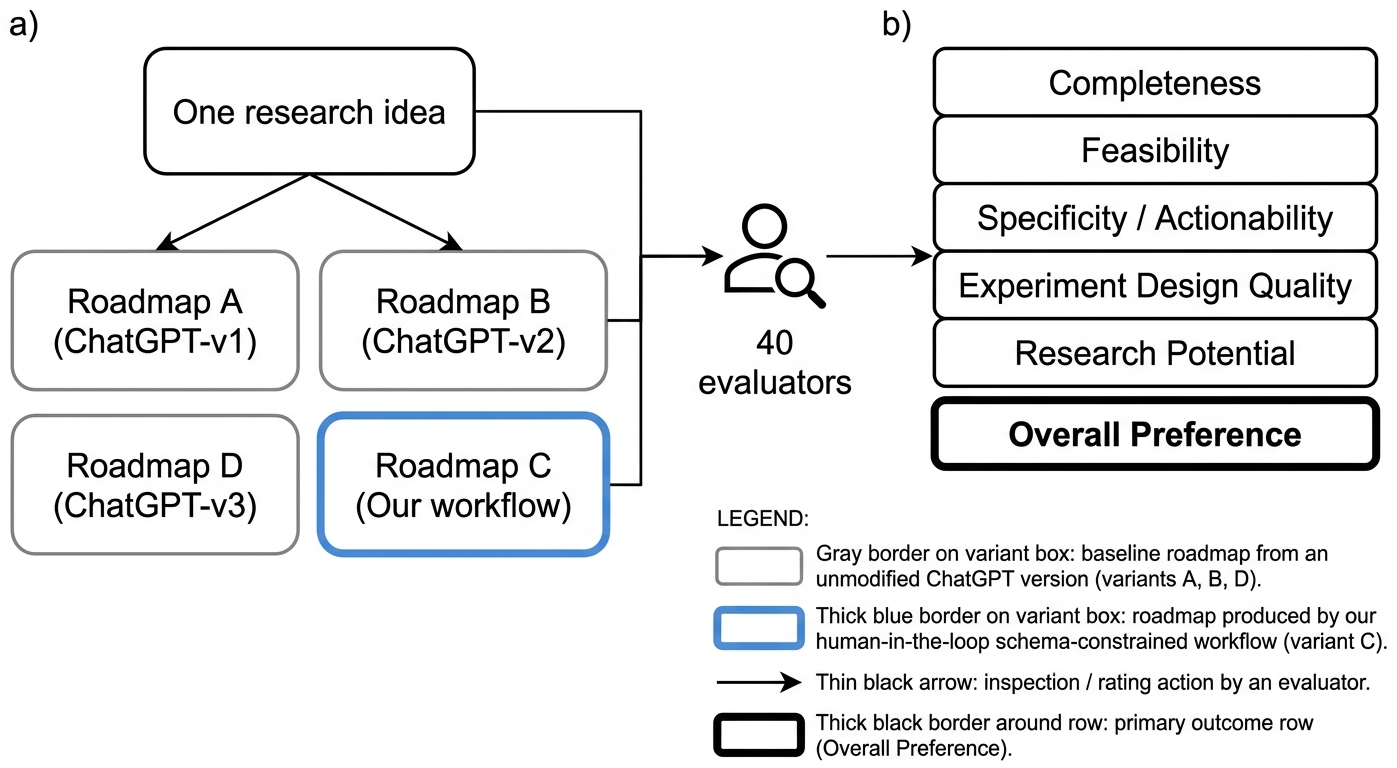
\includegraphics[width=0.95\linewidth]{figures/fig-study-design.png}
  \caption{Study design. For one research idea, four anonymized roadmap
  variants are produced (A, B, D from three different unmodified
  ChatGPT versions; C from our human-in-the-loop schema-constrained
  workflow). Forty evaluators rate every variant on five quality
  dimensions and record a single overall preference. The overall
  preference row is the primary outcome.}
  \label{fig:fig-study-design}
\end{figure}

\subsection{Materials: Roadmap Variants}
\label{sec:eval:materials}

For each research idea we produce four roadmap variants, labeled
\emph{A}, \emph{B}, \emph{C}, and \emph{D}. Variants A, B, and D are
generated by three different unmodified ChatGPT versions, each prompted
in an unstructured way (a single free-form instruction asking for a
research roadmap on the given idea, with no schema and no review loop).
Variant C is produced by our workflow: schema-constrained generation,
optional reference templates, asynchronous compilation to a reviewable
PDF artifact, and one or more human-review iterations through the
\textsf{revision\_requested} state described in
Section~\ref{sec:method:backend}.

The four variants are formatted identically before they reach an
evaluator. Provenance metadata, generator name, model version, and any
other identifying header is stripped, so an evaluator sees only the
roadmap content under the labels \emph{Roadmap A}, \emph{Roadmap B},
\emph{Roadmap C}, and \emph{Roadmap D}. The mapping between labels and
generators is held fixed within the study; we did not randomize letter
order across evaluators in this round, so the labels are consistent but
the labels themselves carry no provenance information.

\subsection{Participants}
\label{sec:eval:participants}

We recruited $40$ evaluators drawn from a research bootcamp cohort,
composed of students, mentors, and adjacent practitioners. Every
evaluator inspected all four roadmap variants for the shared research
idea. Evaluators completed the survey independently and were not given
the identity of any generator before submitting their ratings.

\subsection{Rated Dimensions and Survey Instrument}
\label{sec:eval:dimensions}

Each evaluator rates every variant on five dimensions chosen for
\emph{executability} rather than fluency or helpfulness:

\begin{itemize}
    \item \textbf{Completeness.} Does the roadmap cover research
    questions, methodology, datasets, baselines, metrics, milestones,
    risks, and deliverables?
    \item \textbf{Feasibility.} Can the roadmap be executed within the
    proposed timeline, given accessible datasets or tools, realistic
    milestones, and achievable deliverables?
    \item \textbf{Specificity / Actionability.} Does the roadmap make
    it clear what to read, build, test, compare, and submit?
    \item \textbf{Experiment Design Quality.} Does the experimental
    plan have suitable baselines, measurable metrics, ablations, a
    validation strategy, and clear success criteria?
    \item \textbf{Research Potential.} Does the roadmap have a clear
    problem, plausible novelty, meaningful evaluation, and a realistic
    minimum viable claim, such that the project could plausibly support
    a paper, workshop submission, or technical report?
\end{itemize}

For each dimension, the evaluator selects one variant (out of four) as
the strongest. After completing the per-dimension items, the evaluator
records a single \emph{overall preference}: which roadmap they would
actually adopt and execute. The overall preference is the primary
outcome of the study. Evaluators also provide free-text feedback on why
they selected the strongest roadmap, which roadmap they considered
weakest, and what changes they would request before using the roadmap.

\subsection{Analysis Plan}
\label{sec:eval:analysis}

The primary statistic is the count of overall-preference votes received
by each variant, out of $40$. We test the null hypothesis of uniform
preference across the four variants ($p_0 = 0.25$ per variant) with a
one-sided binomial test on the count of votes received by the
top-ranked variant. Per-dimension counts are reported when available;
in the present round, per-dimension counts were collected at lower
granularity than the overall preference vote, so we treat the
dimension-level evidence as qualitative and rely on the free-text
justifications to characterize \emph{why} evaluators preferred or
rejected a given variant. Section~\ref{sec:results} reports the
results, and Section~\ref{sec:limitations} discusses the threats to
validity that follow from this design.

\section{Results}
\label{sec:results}

\subsection*{Study Setup and Variants}
We collected human preference judgments from $40$ evaluators comparing
four anonymized roadmap variants for the same research idea, labeled
\textbf{A}, \textbf{B}, \textbf{C}, and \textbf{D}. Variants A, B, and D
were generated by three different unmodified ChatGPT versions using a
single unstructured prompt per idea, while \textbf{Variant C} was
produced by our human-in-the-loop, schema-constrained workflow. Each
evaluator inspected all four roadmaps blind to provenance and rated
them on the five dimensions defined in Section~\ref{sec:eval}:
completeness, feasibility, specificity and actionability, experiment
design quality, and research potential. After scoring the per-dimension
items the evaluator was asked which roadmap they would adopt overall.

\subsection*{Overall Preference}
The headline result is concentrated and one-sided. Of the $40$
evaluators, \textbf{$34$ ($85\%$)} selected \textbf{Variant C}, the
roadmap produced by our workflow, as the one they would actually use to
scope and execute the project. The remaining $6$ ($15\%$) preferences
were distributed among the three unstructured-prompt baselines A, B,
and D. Figure~\ref{fig:fig-overall-preference} visualizes the split,
and Table~\ref{tab:overall} reports the count and share for each
variant. A simple majority test rejects the null of uniform preference
among the four variants ($p < 10^{-3}$ under a one-sided binomial test
against $p_0 = 0.25$).

\begin{figure}[t]
  \centering
  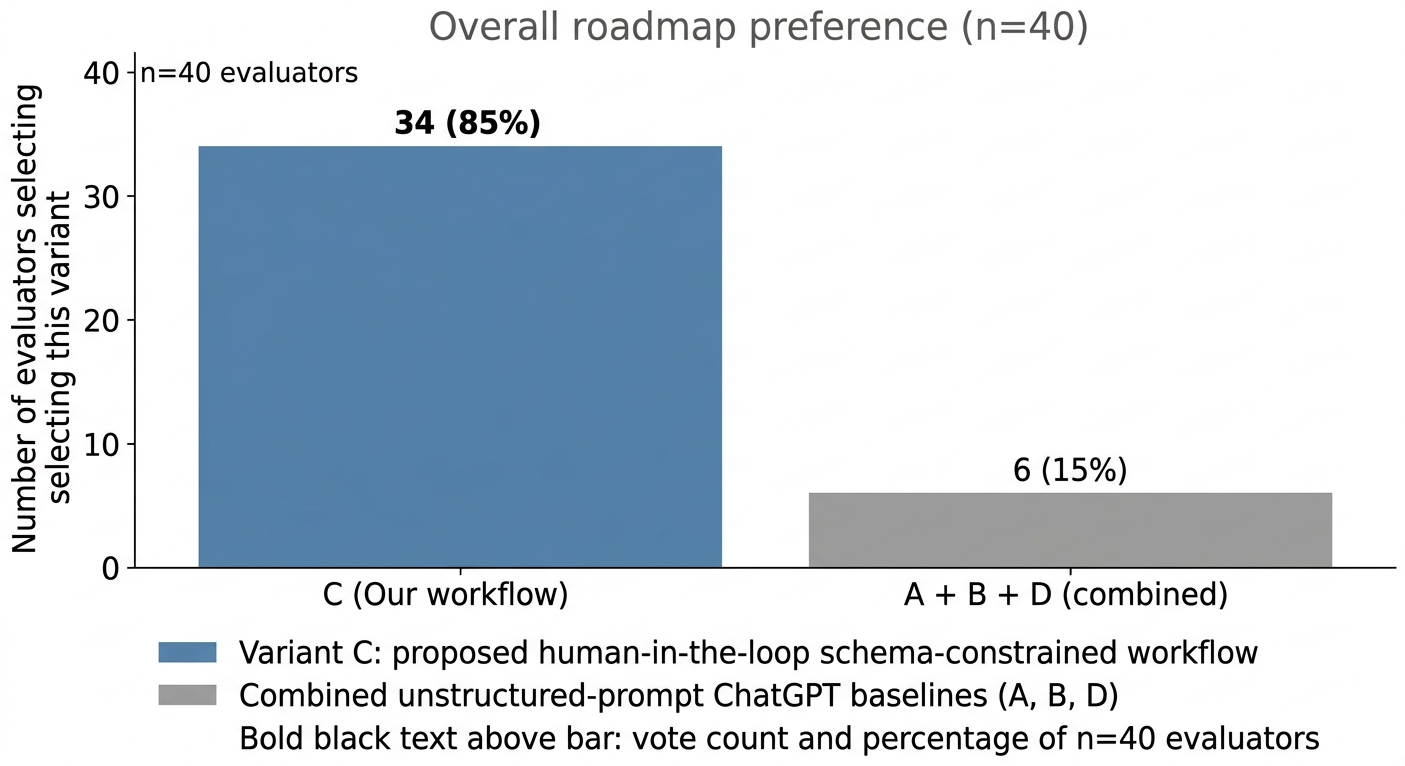
\includegraphics[width=0.95\linewidth]{figures/fig-overall-preference.png}
  \caption{Overall roadmap preference across $40$ evaluators. Variant C
  (the human-in-the-loop, schema-constrained workflow) is selected by
  $34$ of $40$ evaluators ($85\%$); the three unstructured ChatGPT
  baselines A, B, and D collectively receive $6$ votes ($15\%$).}
  \label{fig:fig-overall-preference}
\end{figure}

\begin{table*}[t]
\centering
\begin{tabular}{lcc}
\toprule
Variant & Generator & Overall preference (of $40$) \\
\midrule
A & ChatGPT, unstructured prompt & \multirow{3}{*}{$6$ combined ($15\%$)} \\
B & ChatGPT, unstructured prompt &  \\
D & ChatGPT, unstructured prompt &  \\
\textbf{C (ours)} & \textbf{Schema + human-review workflow} & $\mathbf{34\ (85\%)}$ \\
\bottomrule
\end{tabular}
\caption{Overall roadmap preference across $40$ evaluators. Variant C is the output of the proposed human-in-the-loop schema-constrained workflow; A, B, and D are roadmaps produced by three different unmodified ChatGPT versions for the same idea. Lower-preference variants are reported as a combined count because individual A/B/D shares were not separately captured in the survey instrument.}
\label{tab:overall}
\end{table*}

\subsection*{Per-Dimension Behavior}
Across the five rated dimensions, completeness, feasibility, specificity
and actionability, experiment design quality, and research potential,
our impression from inspecting evaluator comments at the time of
the survey is that the structured roadmap's explicit components
(research questions, baselines, metrics, ablations, weekly milestones,
and a stated minimum viable claim) were the most frequently cited
reason to prefer Variant C, and that the unstructured baselines were
most often criticized for missing or under-specified baselines and
metrics, vague milestones, and overconfident contribution claims. We
deliberately frame this as a researcher impression rather than a
finding because the survey instrument did not retain free-text answers
at the granularity required for direct quotation or reproducible
qualitative coding; we note this as a limitation in
Section~\ref{sec:limitations}. We did not record per-dimension vote
counts at sufficient granularity to report a separate winner for each
dimension; we therefore restrict the quantitative claim to the overall
preference and treat the dimension-level evidence as qualitative.

\subsection*{What the Numbers Do and Do Not Show}
The $34/40$ preference is a measurement of \emph{evaluator-perceived}
roadmap quality at generation time, not of downstream project success.
The result is consistent with our hypothesis that schema-constrained
generation paired with human review produces roadmaps that are more
complete and more actionable than one-shot prompting, but it does not
establish that students who follow Variant C produce stronger final
papers, finish milestones faster, or require fewer mentor interventions.
Section~\ref{sec:limitations} discusses these threats to validity in
detail. We also note that all four variants were generated for a fixed
set of research ideas drawn from a single bootcamp cohort, so the
absolute share favoring Variant C should be read as an effect size on
this evaluator population rather than a population-wide estimate.

\section{Discussion}
\label{sec:discussion}

Research roadmap curation sits between brainstorming and execution. It
is not the same as idea generation, literature review, code generation,
or paper writing; it is the stage where an idea becomes operational.
Many discussions of LLMs in research focus on whether models can write
papers, generate hypotheses, or act as autonomous scientists. Our
framing is narrower and more practical. We do not claim that an LLM can
determine scientific truth or independently supervise research. We find
that an LLM, when constrained by a schema and placed inside a human
review loop, can help produce better first-pass research plans, and the
$34/40$ overall preference for the workflow's roadmap is consistent
with that finding.

The model-agnostic design matters in practice. The contribution is not
tied to a specific backend; different bootcamps, labs, or research
programs can instantiate the same workflow using different LLMs,
templates, review policies, or output formats. What stays fixed is the
structure: schema-constrained generation, reviewable artifacts, an
explicit revision-or-approve decision point, and a human accountable
for the final plan. The asynchronous job lifecycle in
Section~\ref{sec:method:backend} is one realization of that structure;
others are possible, including synchronous web interfaces, terminal
workflows, and editor extensions, as long as the
\textsf{revision\_requested} state remains a first-class concept.

\section{Limitations}
\label{sec:limitations}

The study has several limitations that bound the strength of the
$34/40$ result.

First, human preference at generation time is not downstream project
success. Evaluators who select Variant C are reporting which roadmap
they would adopt, not which roadmap leads to the strongest final paper,
the fastest milestone completion, or the smallest number of mentor
interventions. The next round of work needs to track those downstream
outcomes directly.

Second, the evaluation depends on evaluator expertise. Beginners may
prefer detailed roadmaps that experts find unrealistic, while experts
may penalize roadmaps for missing domain-specific subtleties. Our
$40$-evaluator cohort was drawn from a research bootcamp and includes
students, mentors, and adjacent practitioners; the absolute share
favoring Variant C should therefore be read as an effect size on this
population rather than a population-wide estimate.

Third, the same roadmap schema may not work equally well across
domains. A roadmap for reinforcement learning, scientific machine
learning, multimodal retrieval, or AI-systems work may require
different levels of detail and different default components. The schema
in Figure~\ref{fig:fig-schema} is intentionally coarse-grained, but a
domain-specific instantiation may push more components into the
methodology family.

Fourth, the workflow may inherit biases from the reference templates
that condition generation. If the templates emphasize certain styles
of project, the generated roadmaps may overproduce similar structures.
We did not control for this in the present study.

Fifth, the labels A, B, C, and D were held fixed across evaluators
rather than randomized per evaluator, so any latent label bias (for
example, evaluators tending to read C more carefully because it sits
in the middle of the list) would inflate the apparent preference for
C. A future round should randomize label-to-variant mapping
per evaluator and report the same primary outcome under that design.

Sixth, the survey instrument captured the overall preference at higher
granularity than the per-dimension votes; this is why
Section~\ref{sec:results} reports the dimension-level evidence as
qualitative rather than as five separate counts. A revised survey
should record per-dimension votes at the same granularity as the
overall preference so each dimension can be tested independently.

Seventh, the study uses a single shared research idea across all four
roadmap variants. Holding the topic fixed controls for idea preference
within the comparison, but it also means the $34$ of $40$ overall
preference reported here is conditional on that one idea. The effect
size could be inflated, attenuated, or reversed for ideas that are
narrower, more domain-specific, or more poorly matched to the
workflow's reference templates. A $k$-idea generalization, with the
same blind protocol applied to multiple ideas drawn from different
subareas, is required before the result can be read as a population
claim about idea-to-roadmap conversion in general. We acknowledge this
as the most consequential limitation of the present round.


\section{Conclusion}
\label{sec:conclusion}

We presented a human-in-the-loop LLM workflow for research roadmap
curation. The workflow converts vague research ideas into structured,
reviewable execution plans containing research questions, literature
directions, datasets, baselines, metrics, ablations, risks, milestones,
deliverables, and a minimum viable claim, and it places a human
reviewer at an explicit \textsf{revision\_requested} decision point
rather than only at the prompt. In a blind preference study with $40$
evaluators rating four anonymized roadmap variants for one shared
research idea, \textbf{$34$ ($85\%$)} selected the workflow's roadmap
as the one they would adopt, against $6$ for the three unstructured
ChatGPT baselines. The single-idea design means the absolute share
should be read as conditional on the chosen idea, not as a
population-wide estimate.

The result is consistent with, but does not by itself establish, the
broader claim that schema-constrained generation under human review
produces more usable first-pass research plans than one-shot
prompting. Two natural follow-ups are most useful. First,
\emph{downstream evaluation}: track whether participants who execute a
Variant-C roadmap actually finish more milestones on time, write
stronger reports, or require fewer mentor interventions than those who
follow an unstructured roadmap. Second, \emph{domain-specific schemas}:
adapt the twelve-component schema to the conventions of specific
research subareas and re-run the preference study against each
domain's expert evaluators. The value of LLMs in early-stage research
planning is not autonomous research generation, but structured
assistance under human oversight, and we expect the operational
benefits to grow as the structure and the oversight become more
specific to the domain.

\FloatBarrier
\bibliographystyle{icml2024}
\bibliography{references}

\end{document}
